\section{Bảng chân trị}
Để thiết kế mạch đèn Led 7 Đoạn gồm 4 đầu vào và 7 đầu ra (tương ứng với 7 đoạn của đèn led). Các đoạn đèn led sẽ hiển thị con số tương ứng với 4 bit đầu vào.

\begin{figure}[H]
	\centering
	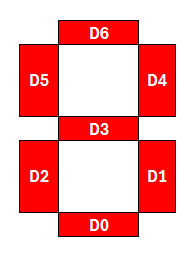
\includegraphics[width=0.3\textwidth]{images/img0.PNG}
	\caption{Mạch đèn Led 7 đoạn}
	\label{fig:7segment}
\end{figure}

Để thiết kế mạch này, ta cần xác định bảng chân trị cho 7 đoạn led. Bảng chân trị này sẽ giúp ta xác định cách kết nối các đoạn led với các bit đầu vào. Bảng chân trị cho 7 đoạn led được mô tả như sau:

Các đầu vào của mạch là $I_3, I_2, I_1, I_0$ và các đầu ra là $D_6, D_5, D_4, D_3, D_2, D_1, D_0$.

Số 0 dưới dạng nhị phân là 0000, sẽ bật các đoạn LED: \(D_0, D_1, D_2, D_4, D_5, D_6\)  và tắt các đoạn LED: \(D_3\).

Số 1 dưới dạng nhị phân là 0001, sẽ bật các đoạn LED: \(D_1, D_4\) và tắt các đoạn LED: \(D_0, D_2, D_3, D_5, D_6\).

Số 2 dưới dạng nhị phân là 0010, sẽ bật các đoạn LED: \(D_0, D_2, D_3, D_4, D_6\) và tắt các đoạn LED: \(D_1, D_5\).

Số 3 dưới dạng nhị phân là 0011, sẽ bật các đoạn LED: \(D_0, D_1, D_3, D_4, D_6\) và tắt các đoạn LED: \(D_5, D_2\).

Số 4 dưới dạng nhị phân là 0100, sẽ bật các đoạn LED: \(D_1, D_3, D_4, D_5\) và tắt các đoạn LED: \(D_0, D_2, D_6\).

Số 5 dưới dạng nhị phân là 0101, sẽ bật các đoạn LED: \(D_0, D_1, D_3, D_5, D_6\) và tắt các đoạn LED: \(D_2, D_4\).

Số 6 dưới dạng nhị phân là 0110, sẽ bật các đoạn LED: \(D_0, D_1, D_2, D_3, D_5, D_6\) và tắt các đoạn LED: \(D_4\).

Số 7 dưới dạng nhị phân là 0111, sẽ bật các đoạn LED: \(D_1, D_4,  D_6\) và tắt các đoạn LED: \(D_0, D_2, D_3, D_5\).

Số 8 dưới dạng nhị phân là 1000, sẽ bật tất cả các đoạn LED: \(D_0, D_1, D_2, D_3, D_4, D_5, D_6\).

Số 9 dưới dạng nhị phân là 1001, sẽ bật các đoạn LED: \(D_0, D_1, D_3, D_4, D_5, D_6\) và tắt các đoạn LED: \(D_2\).

Bảng chân trị cho mạch đèn Led 7 đoạn được vẽ như sau:

\renewcommand{\arraystretch}{1.5}

\[
	\begin{array}{|>{\Large}c|>{\Large}c|>{\Large}c|>{\Large}c||>{\Large}c|>{\Large}c|>{\Large}c|>{\Large}c|>{\Large}c|>{\Large}c|>{\Large}c|}
		\hline
		I_3 & I_2 & I_1 & I_0 & D_6 & D_5 & D_4 & D_3 & D_2 & D_1 & D_0 \\
		\hline
		0   & 0   & 0   & 0   & 1   & 1   & 1   & 0   & 1   & 1   & 1   \\
		\hline

		0   & 0   & 0   & 1   & 0   & 0   & 1   & 0   & 0   & 1   & 0   \\
		\hline

		0   & 0   & 1   & 0   & 1   & 0   & 1   & 1   & 1   & 0   & 1   \\
		\hline

		0   & 0   & 1   & 1   & 1   & 0   & 1   & 1   & 0   & 1   & 1   \\
		\hline

		0   & 1   & 0   & 0   & 0   & 1   & 1   & 1   & 0   & 1   & 0   \\
		\hline

		0   & 1   & 0   & 1   & 1   & 1   & 0   & 1   & 0   & 1   & 1   \\
		\hline

		0   & 1   & 1   & 0   & 1   & 1   & 0   & 1   & 1   & 1   & 1   \\
		\hline

		0   & 1   & 1   & 1   & 1   & 0   & 1   & 0   & 0   & 1   & 0   \\
		\hline

		1   & 0   & 0   & 0   & 1   & 1   & 1   & 1   & 1   & 1   & 1   \\
		\hline

		1   & 0   & 0   & 1   & 1   & 1   & 1   & 1   & 0   & 1   & 1   \\
		\hline
	\end{array}
\]